\documentclass[12pt,a4paper]{report}
\usepackage[a4paper, total={6in, 9.5in}]{geometry}
\usepackage[pdftex]{graphicx} %for embedding images
\usepackage{url} %for proper url entries
\usepackage[backend=biber]{biblatex}
\usepackage{float}
\usepackage{algpseudocode}
\usepackage{algorithm}
\usepackage{setspace}
\usepackage{ragged2e}

\usepackage{hyperref}
\hypersetup{
	colorlinks=true, %set true if you want colored links
	linktoc=all,     %set to all if you want both sections and subsections linked
	linkcolor=black,  %choose some color if you want links to stand out
}

\usepackage{listings}   %configuration for codes
\usepackage{colortbl}

\usepackage{multirow}
\usepackage{graphicx}
\usepackage[table,xcdraw]{xcolor}
\usepackage{ulem}

\definecolor{codegreen}{rgb}{0,0.6,0}
\definecolor{codegray}{rgb}{0.5,0.5,0.5}
\definecolor{codepurple}{rgb}{0.58,0,0.82}
\definecolor{backcolour}{rgb}{0.95,0.95,0.92}

\lstdefinestyle{plain}{
	backgroundcolor=\color{backcolour},   
	numberstyle=\tiny\color{codegray},
	basicstyle=\ttfamily\scriptsize,
	breakatwhitespace=false,         
	breaklines=true,                 
	keepspaces=true,                 
	numbers=left,       
	numbersep=5pt,                  
	showspaces=false,                
	showstringspaces=false,
	showtabs=false,                  
	tabsize=2
}

\lstdefinestyle{Terminal}{
	language=bash,
	backgroundcolor=\color{backcolour},   
	commentstyle=\color{codegreen},
	keywordstyle=\color{magenta},
	numberstyle=\tiny\color{codegray},
	stringstyle=\color{codepurple},
	basicstyle=\ttfamily\scriptsize,
	breakatwhitespace=false,         
	breaklines=true,                 
	keepspaces=true,                 
	numbers=left,       
	numbersep=5pt,                  
	showspaces=false,                
	showstringspaces=false,
	showtabs=false,                  
	tabsize=2
}

\lstdefinestyle{CStyle}{
	language=C,
	backgroundcolor=\color{backcolour},   
	commentstyle=\color{codegreen},
	keywordstyle=\color{magenta},
	numberstyle=\tiny\color{codegray},
	stringstyle=\color{codepurple},
	basicstyle=\ttfamily\scriptsize,
	breakatwhitespace=false,         
	breaklines=true,                 
	keepspaces=true,                 
	numbers=left,       
	numbersep=5pt,                  
	showspaces=false,                
	showstringspaces=false,
	showtabs=false,                  
	tabsize=2
}

\begin{document}
\renewcommand\bibname{References} 
%Renames "Bibliography" to "References" on ref page

\renewcommand{\contentsname}{List of Experiments}

\renewcommand{\chaptername}{Experiment}

%include other pages
\begin{titlepage}
	\clearpage
	\vspace*{\fill}
	\thispagestyle{empty}
	\begin{onehalfspace}
	\begin{center}
			
		\textup{\large{\bf CS431 Compiler Design Lab Record}}
		\\[0.2in]
		
       \small \emph{Submitted in partial fulfillment of\\ the requirements for the award of the degree of}
		\vspace{.2in}
		{\bf Bachelor of Technology \\in\\ Computer Science and Engineering}\\[0.5in]
		
		% Submitted by
		\normalsize Submitted by \\
		\begin{table}[h]
			\centering
			\begin{tabular}{cc}
				KTU Register No & Name of Student
				\\ \hline \\
				rollno      & Edwin Jose George
			\end{tabular}
		\end{table}
		
		\vspace{.1in}
		Faculty-in-charge(s)\\ [0.1in]
		\textbf{Faculty1}\\ 
		FacultyTitle\\ [0.1in]
		\textbf{Faculty2}\\
		FacultyTitle \\ [0.2in]
		
		\vfill
	
		% Bottom of the page
		
\includegraphics[width=0.2\textwidth]{./gcek_logo.jpg}\\[0.1in]
		\Large{Department of Computer Science and Engineering}\\
		\normalsize \textsc{Government College of Engineering Kannur}\\ Kannur, Kerala, India -- 670563 \\
		\vspace{0.2cm}
	
	\end{center}
	\end{onehalfspace}
	\vspace*{\fill}
\end{titlepage}

\newpage
\thispagestyle{empty}
\vspace*{\fill}
\begin{onehalfspace}
\begin{center}

	\huge{Department of Computer Science and Engineering}\\[0.5cm]
	\normalsize \textsc{Government College of Engineering Kannur}\\[2.0cm]

	\emph{\LARGE Certificate}\\[1.0cm]
\end{center}

\normalsize This is to certify that this is a bonafide record of CS334 Network Programming Lab work done by the student whose name is given below in partial fulfillment of the requirements of the degree of Bachelor of Technology in Computer Science and Engineering under A.P.J.Abdul Kalam Technological University during the year 2021-22.\\[1.0cm]

\begin{table}[h]
	\centering
	\begin{tabular}{cc}
		KTU Register No & Name of Student
		\\ \hline \\
		KNR18CS027      & Edwin Jose George
	\end{tabular}
\end{table}
\vspace{2cm}


\begin{table}[h]
	\centering
	\makebox[\linewidth]{
		\begin{tabular}{ccc}
			Faculty-in-charge & Faculty-in-charge & H.o.D \\ \\
			Prof. Dileep M R & Prof. Sajith.B &  Dr.Rafeeque P. C. \\
			(Asst Professor,CSE Dept.) & (Asst Professor,CSE Dept.) & (Prof and H.o.D,CSE Dept.)\\
		\end{tabular}
	}
\end{table}
\end{onehalfspace}
\vspace*{\fill}
% Bottom of the page

\clearpage
\vspace*{\fill}
\begin{onehalfspace}
\begin{center} 
	\section*{Institute Vision}
	\begin{justify}
	``A globally renowned institution of excellence in engineering, education, research and consultancy.''
	\end{justify}
			
	\section*{Institute Mission}
	\begin{justify}
	``To contribute to the society by providing quality education and training, leading to innovation, entrepreneurship and sustainable growth.''
	\end{justify}
			
	\section*{Department Vision}
	\begin{justify}
	``To be a centre of excellence in the field of Computer Science \& Engineering education and research, which extends its appreciated services to the industry and the society.''
	\end{justify}
			
	\section*{Department Mission}
	\begin{justify}
	``To develop engineers with excellent analytic, design and implementation skills, who can expertise themselves as computer professionals, research engineers, entrepreneurs or as managers, while fulfilling their ethical and social responsibilities, in a globally competitive environment.''
	\end{justify}
\end{center}
\end{onehalfspace}
\vspace*{\fill}


\pagenumbering{roman} %numbering before main content starts
\setcounter{page}{0}

\tableofcontents

\cleardoublepage
\pagenumbering{arabic} %reset numbering to normal for the main content

\clearpage
\chapter{Lexical analyzer for C language using C language}

\section{Aim}
To design and implement a lexical analyzer for given language using C. The lexical analyzer should ignore redundant spaces, tabs and new lines.

\section{Algorithm}

\begin{figure}[H]
	\centering
	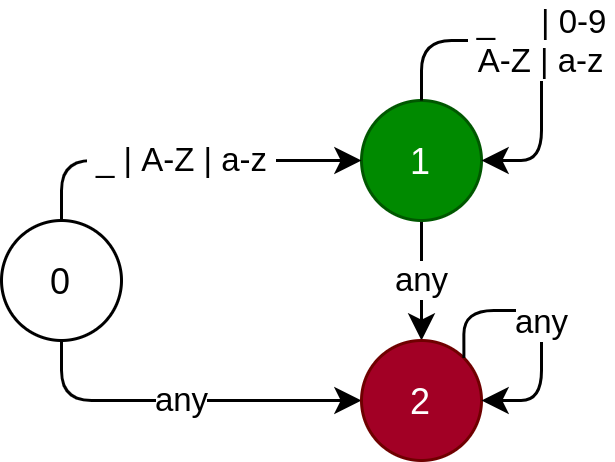
\includegraphics[height=2.5in]{../EXP1/identifier.png}
	\caption{Finite Automaton to detect an identifier.}
\end{figure}

\begin{figure}[H]
	\centering
	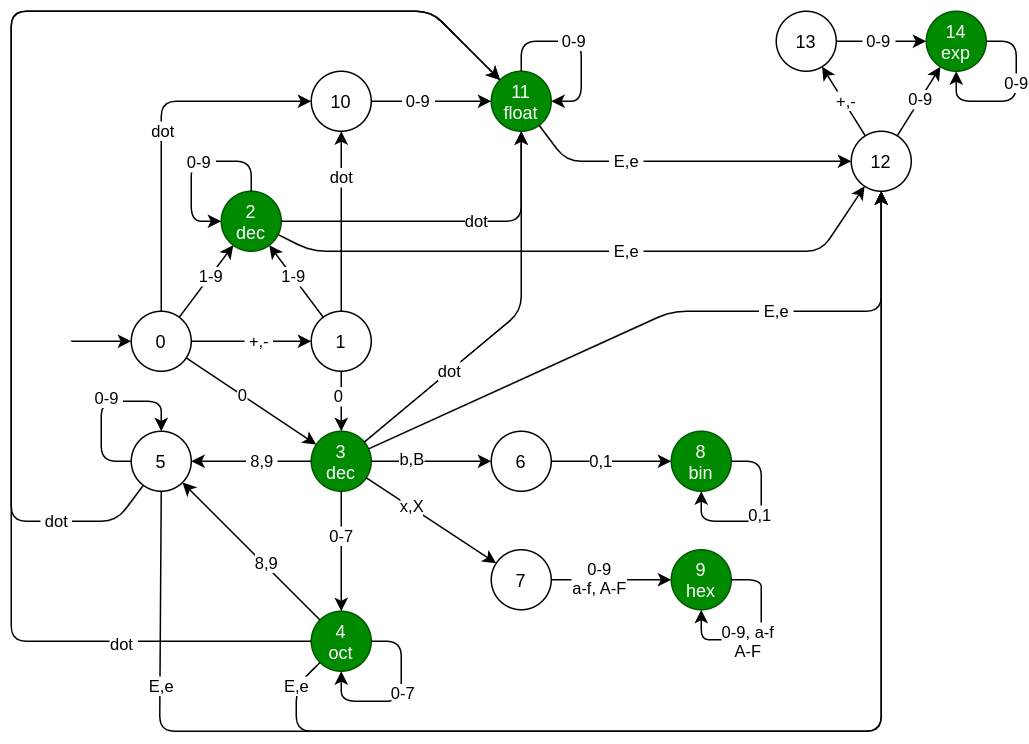
\includegraphics[width=\textwidth]{../EXP1/numerals.png}
	\caption{Finite Automaton to detect an numeral type.}
\end{figure}


\begin{figure}[H]
	\centering
	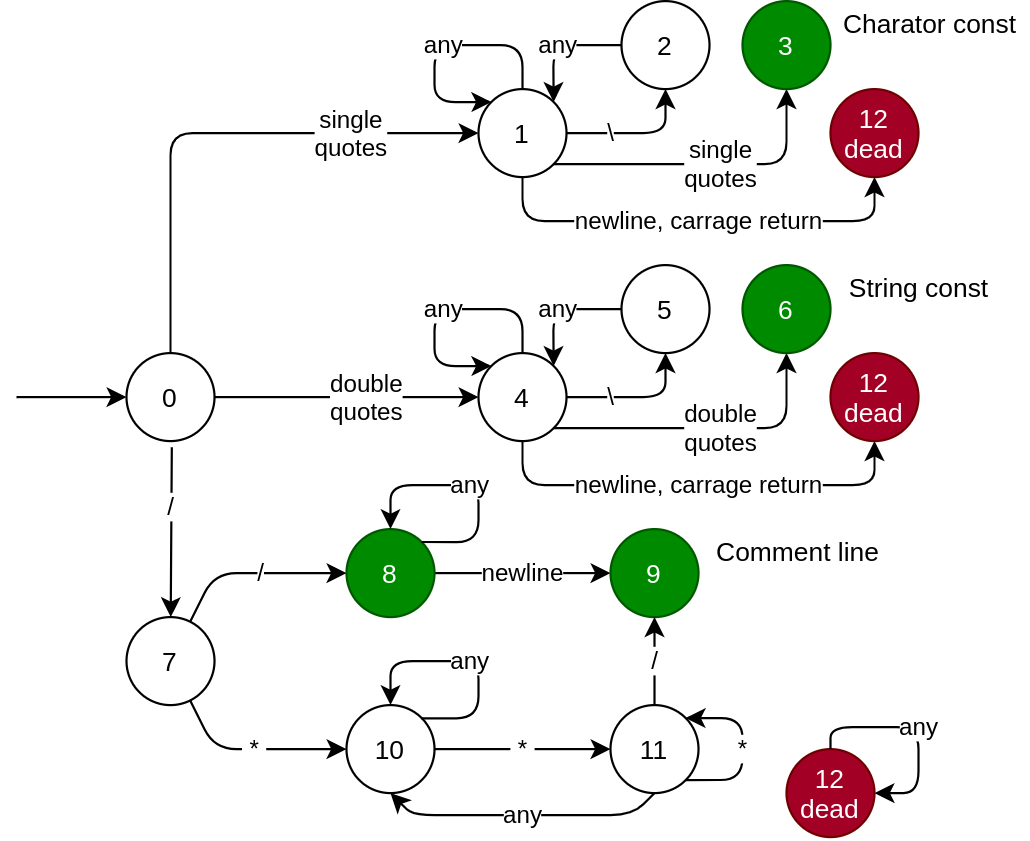
\includegraphics[width=\textwidth]{../EXP1/char-stream.png}
	\caption{Finite Automaton to detect comments, string/char literal and escape sequence}
\end{figure}


\section{C-Program}
Header file \textbf{stack.h} to stimulate stack.
\lstinputlisting[style=CStyle]{../EXP1/stack.h}

\vspace{0.5cm}
Header file \textbf{definition.h} holds various subroutines and constants that aid to analyze lexemes of C language.
\lstinputlisting[style=Cstyle]{../EXP1/definition.h}

\vspace{0.5cm}
C program file \textbf{CLexical.c} initiates and scans lexemes.
\lstinputlisting[style=Cstyle]{../EXP1/CLexical.c}


\section{Output}
C program used for testing \textbf{sample.c}.
\lstinputlisting[style=CStyle]{../EXP1/sample.c}

\vspace{0.5cm}
Lexical analyzer output
\lstinputlisting[style=plain]{../EXP1/sample_out.txt}

\section{Result}
The program compiled successfully and identified various C tokens from the sample C program file. 
\clearpage
\chapter{Lexical analyzer for C language using Lex tool}

\section{Aim}
To design and implement a lexical analyzer for given C language using lex tool. The lexical analyzer should ignore redundant spaces, tabs and new lines.

\section{Algorithm}

\begin{figure}[H]
	\centering
	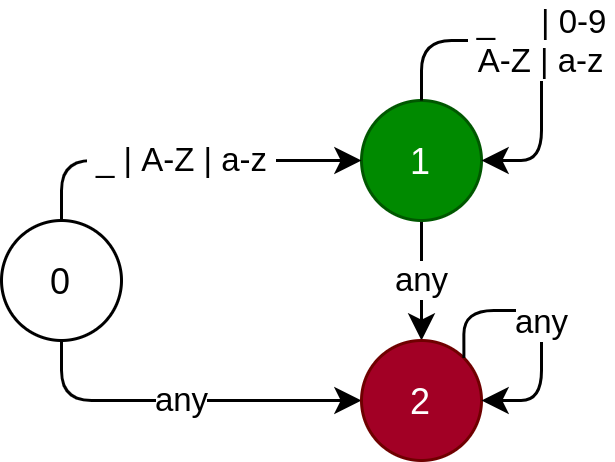
\includegraphics[height=2.5in]{../EXP1/identifier.png}
	\caption{Finite Automaton to detect an identifier.}
\end{figure}

\begin{figure}[H]
	\centering
	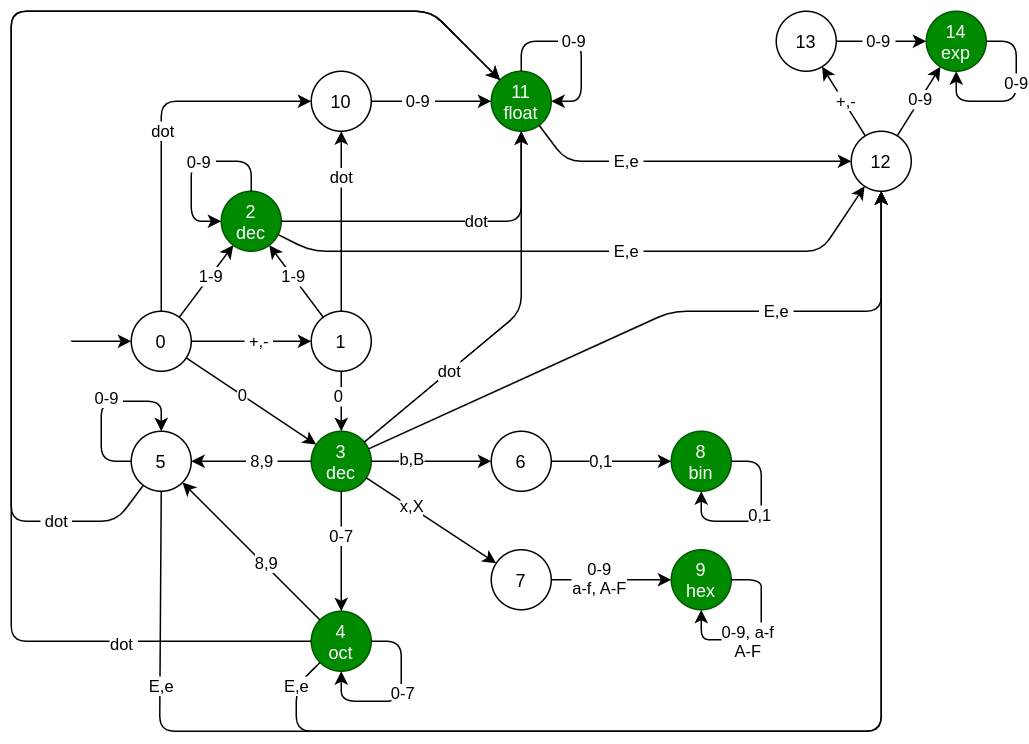
\includegraphics[width=\textwidth]{../EXP1/numerals.png}
	\caption{Finite Automaton to detect an numeral type.}
\end{figure}


\begin{figure}[H]
	\centering
	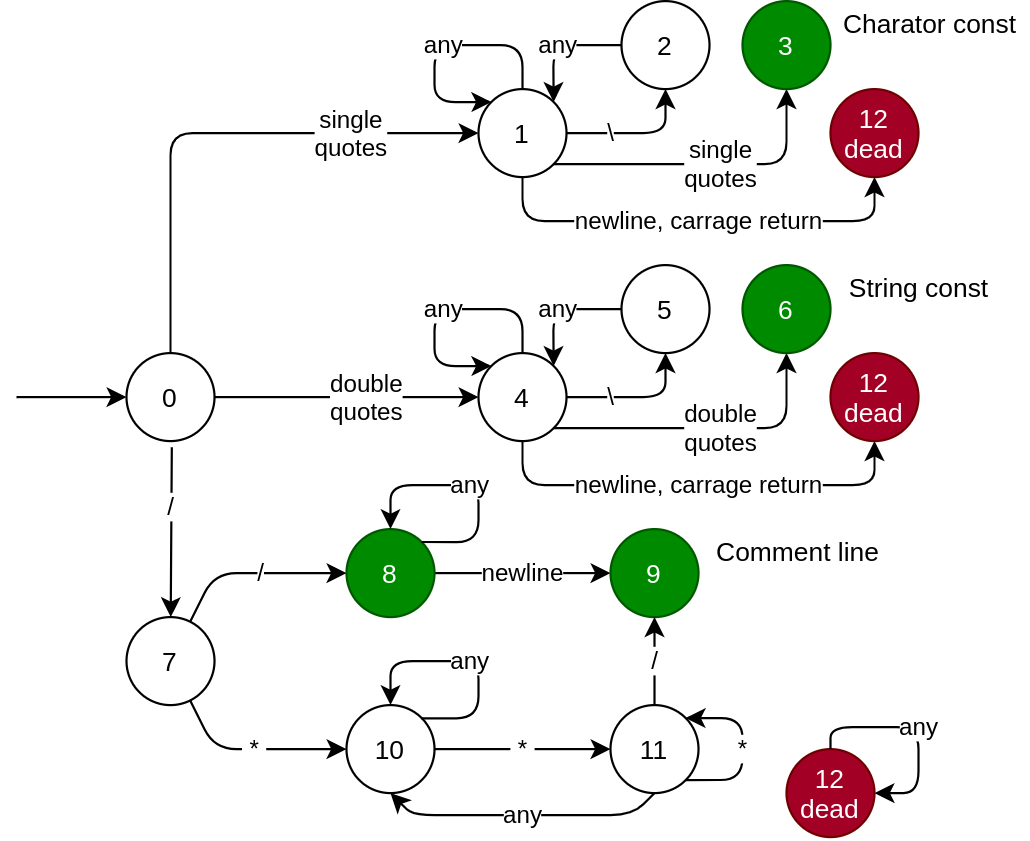
\includegraphics[width=\textwidth]{../EXP1/char-stream.png}
	\caption{Finite Automaton to detect comments, string/char literl and escape sequence}
\end{figure}


\section{C-Program}
Header file \textbf{stack.h} to stimulate stack.
\lstinputlisting[style=CStyle]{../EXP2/stack.h}

\vspace{0.5cm}
Header file \textbf{definition.h} holds various subroutines and constants that aid to analyze keywords and identifiers. The lex tool detects identifers. A table is cross checked to detect keywords.
\lstinputlisting[style=Cstyle]{../EXP2/definition.h}

\vspace{0.5cm}
Lex file \textbf{CLexical.l} initiates and scans lexemes.
\lstinputlisting[style=Cstyle]{../EXP2/CLexical.l}



\section{Output}
C program used for testing \textbf{sample.c}.
\lstinputlisting[style=CStyle]{../EXP2/sample.c}


\vspace{0.5cm}
Compiling lex file
\begin{lstlisting}[style=Terminal]
	$ lex CLexical.l
	$ gcc lex.yy.c
	$ ./a.out sample.c
\end{lstlisting}

\vspace{0.5cm}
Lexical analyser output
\lstinputlisting[style=plain]{../EXP2/sample_out.txt}

\section{Result}
The Lexicial analyser is stimulated successfully and the output is verified.
\clearpage
\chapter{Generation of YACC specification for a few syntactic categories}

\section{Aim}
To design and implement YACC specification for the following syntactic categories.
\begin{enumerate}
	\item Program to recognize a valid arithmetic expression that uses operator +, – , * and /.
	%\item Program to recognize a valid variable which starts with a letter followed by any	number of letters or digits.
	%\item Implementation of Calculator using LEX and YACC
	%\item Convert the BNF rules into YACC form and write code to generate abstract syntax tree
\end{enumerate}


\section{Recognize Arithmetic expression}
\subsection{Algorithm}
\begin{algorithm}[H]
	\caption{An algorithm to recognize numbers , operators and variables}
	\begin{algorithmic}[1]
		\State $isNum \gets False$
		\State $isVar \gets False$
		\State $buf \gets ""$
		\State $i \gets 0$
		\State $buf[i] \gets $ inputChar()
		\While{$buf[i]$ == whitespace}
		\State $buf[i] \gets $ inputChar()
		\EndWhile
		
		\If{ $buf[i]$ == operator }
		\State $return$ $buf[i]$,"operator"
		\ElsIf{ $buf[i]$ == '(' }
		\State $return$ $buf[i]$,"openBracket"
		\ElsIf{ $buf[i]$ == ')' }
		\State $return$ $buf[i]$,"closeBracket"
		\ElsIf{$buf[i]$ == alpha or underscore}
		\State $isVar \gets True$
		\ElsIf{$buf[i]$ == number}
		\State $isNum \gets True$
		\Else
		\State $return$ "ERROR"
		\EndIf
		\State $i \gets i+1$
		
		\While{$(buf[i]$ = inputChar()) $\neq$ EOF}
		\If{$isVar and buf[i]$ == (alphaNum or underscore)}
		\State $i \gets i + 1$
		\State continue
		\ElsIf{$isNum$ and $buf$ == number)}
		\State $i \gets i + 1$
		\State continue
		\Else
		\State unputChar($buf[i]$) \Comment{Put back the last char read}
		\State $buf[i]$ = $'\ '$
		\If{$isVar$}
		\State $return$ $buf$,"variable"
		\ElsIf{$isNum$}
		\State $return$ $buf$,"number"
		\Else
		\State $return$ "ERROR"
		\EndIf
		\EndIf
		\EndWhile
	\end{algorithmic}
\end{algorithm}

\begin{algorithm}[H]
	\caption{A grammar to recognize expression}
	\begin{algorithmic}[1]
		\State $FINAL\_EXPR \gets EXPR$ $NEWLINE$
		\State $EXPR \gets number$
		\State $EXPR \gets identifier$
		\State $EXPR \gets $openBracket $EXPR$ closeBracket
		\State $EXPR \gets EXPR$ operator $EXPR$
	\end{algorithmic}
\end{algorithm}

\subsection{Lex program}
\lstinputlisting[style=CStyle]{../EXP3/expression.l}
\subsection{Yacc Program}
\lstinputlisting[style=CStyle]{../EXP3/expression.y}
\subsection{Output}
Compiling program
\lstinputlisting[style=Terminal]{../EXP3/expression_run.sh}


\vspace{0.5cm}
Output
\lstinputlisting[style=plain]{../EXP3/expression_output.txt}



\section{Result}
Implemented and verified YACC specification for a few syntactic categories
\clearpage
\chapter{Traversing $\epsilon$ transitions in NFA}

\section{Aim}
To design and implement a C-program that accepts a Non-deterministic Finite Automaton (NFA) and computes $\epsilon$ closure for each states.

\section{Algorithm}

\begin{algorithm}[H]
	\caption{An algorithm to compute $\epsilon$ closure of a state}
	\begin{algorithmic}
		\Procedure{findEpsilionTrans}{$visited, fromState$}
		\State \Comment{visited : Stack of visited states}
		\State \Comment{fromState : Current state to find closure}
		
		\If{$fromstate \in visited$}
		\State return $visited$
		\EndIf
		
		\State $push(visited, fromState)$
		
		\ForAll{$transition \in fromState.transitions$}
		\If{$transition.symbol == \epsilon $}
		\State $visited = $ \Call{findEpsilonTrans}{visited, transition.toState}
		\EndIf
		\EndFor
		\EndProcedure
	\end{algorithmic}
\end{algorithm}

\subsubsection*{Realization of NFA using linked list}

\begin{figure}[H]
	\centering
	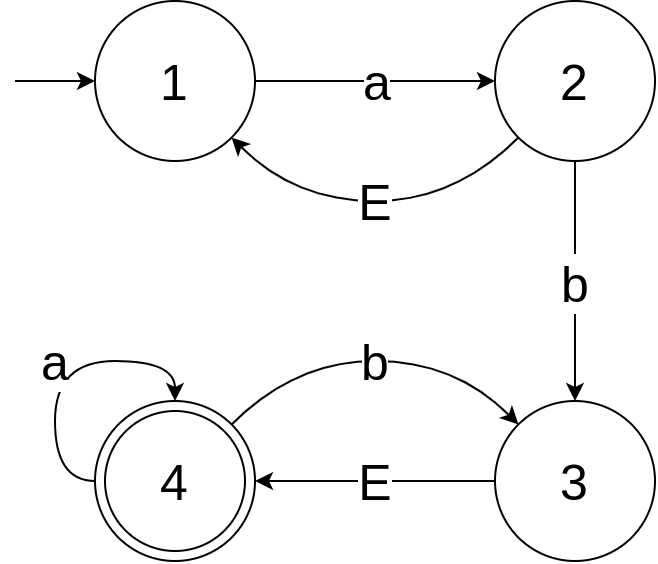
\includegraphics[height=2in]{../EXP4/NFA_realization-NFA.png}
	\caption{NFA}
\end{figure}

\begin{figure}[H]
	\centering
	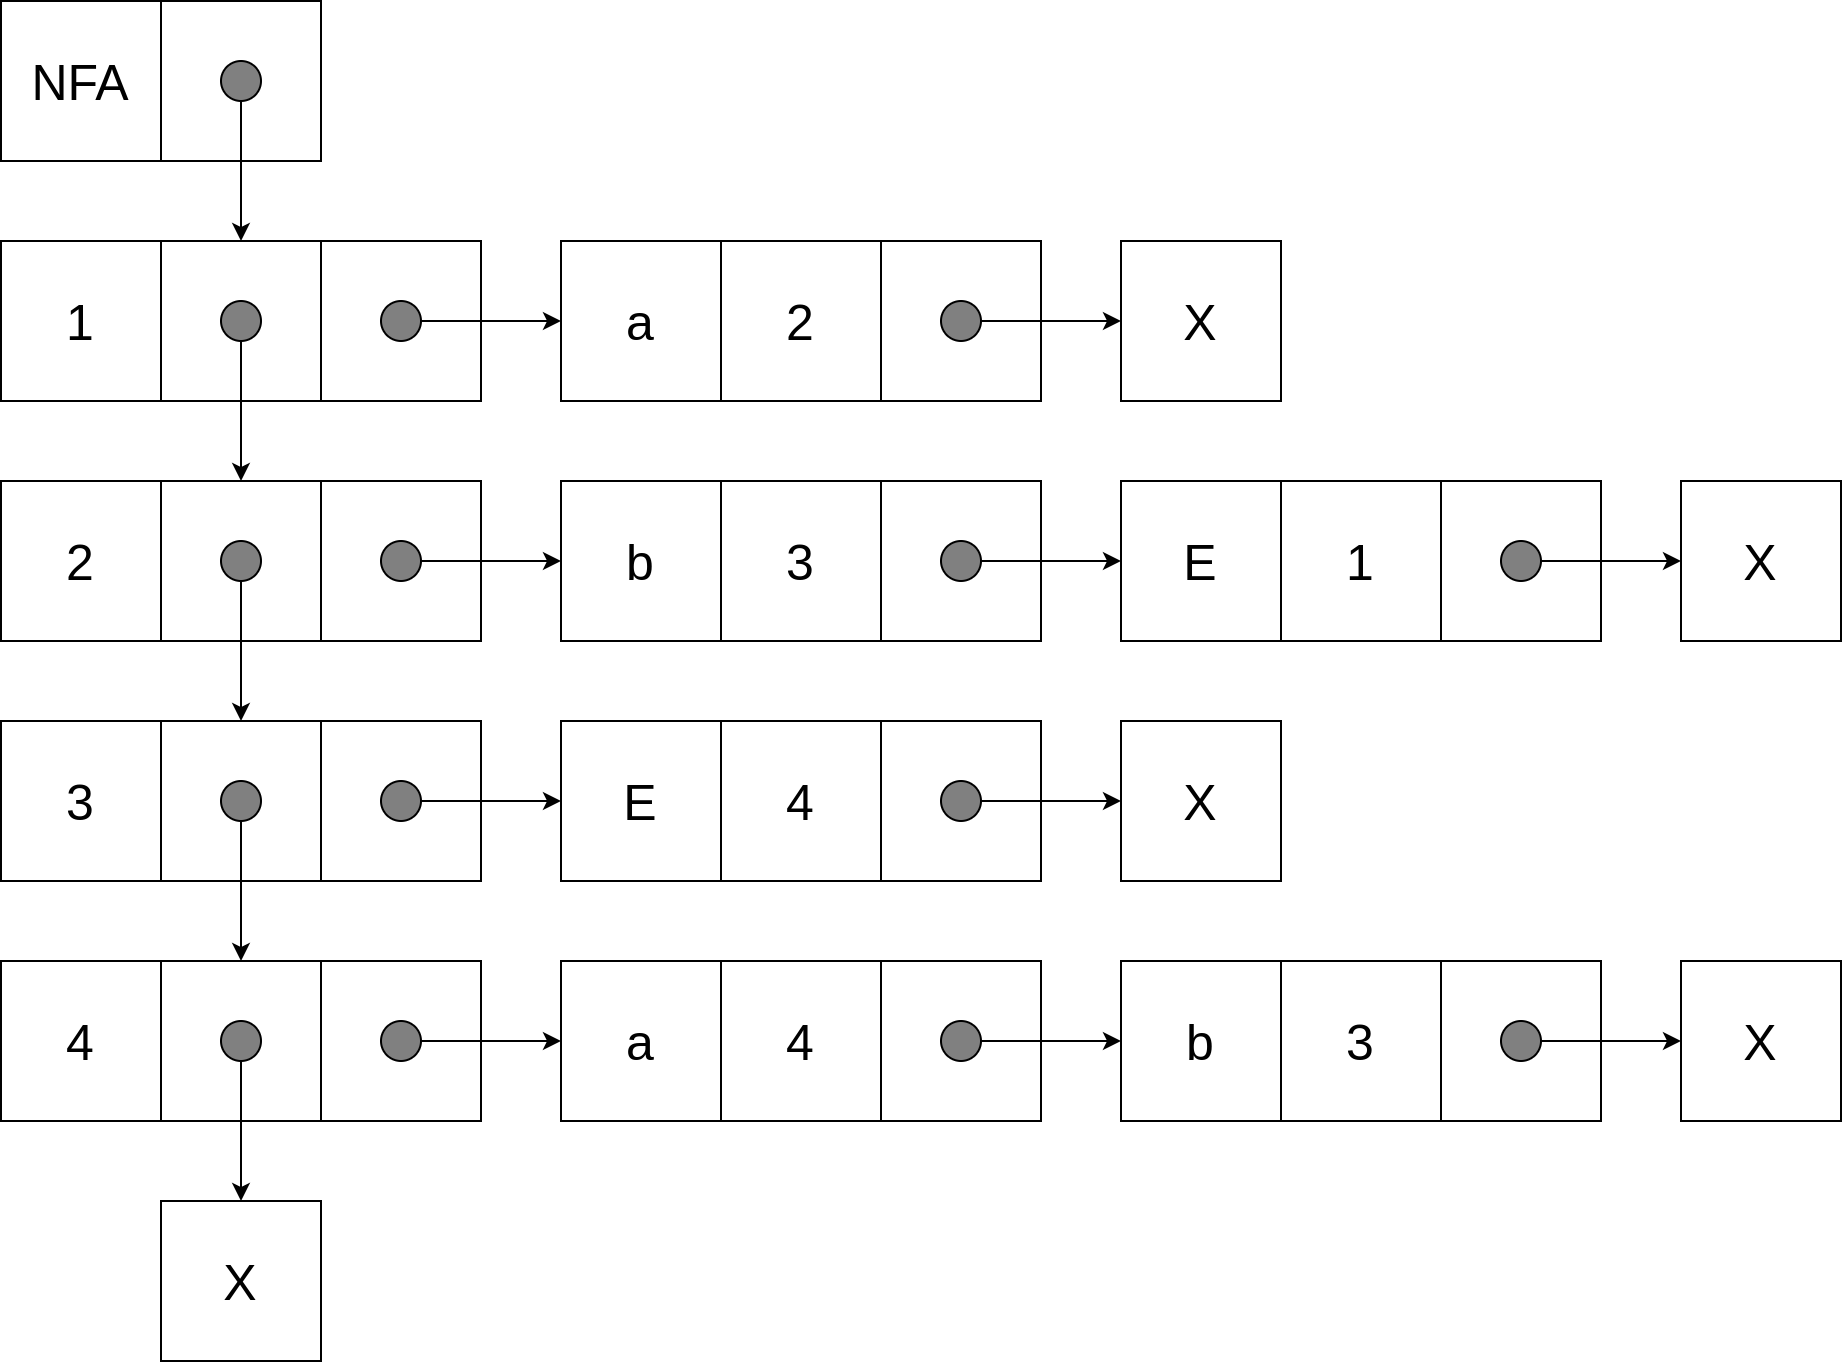
\includegraphics[height=2.5in]{../EXP4/NFA_realization-LinkedList.png}
	\caption{NFA realization via linked list}
\end{figure}
\section{C-Program}
\lstinputlisting[style=CStyle]{../EXP4/epsilonNFA.c}

\section{Output}
\lstinputlisting[style=plain]{../EXP4/output.txt}

\section{Result}
The program compiled successfully and identified $\epsilon$ closure for each states in the given NFA.
\clearpage
\chapter{Converting $\epsilon$-NFA to NFA}

\section{Aim}
To design and implement a program that accepts a Epsilon Non-deterministic Finite Automaton ($\epsilon$-NFA) and computes NFA without $\epsilon$ transitions.

\section{Algorithm}

\begin{algorithm}[H]
	\caption{An algorithm to convert $\epsilon$-NFA to NFA }
	\begin{algorithmic}
		\Procedure{computeTransition}{$state, sym$}
			\State \Comment{state : starting state}
			\State \Comment{inputs : input symbol}
			
			\State $resultSet \gets \{\}$ \Comment{Empty set}
			
			\State $Eset \gets \Call{EClosure}{state}$ \Comment{Computing e-closure}
			
			
			\ForAll{$Estate \in Eset$}
				\State $Tstates \gets \Call{transition}{Estate,sym}$ \Comment{set of states after transition}
				\ForAll{$subState \in Tstates$}
					\State $resultSet \gets resultSet \cup \Call{EClosure}{subState}$ \Comment{Union of eclosures}
				\EndFor
			\EndFor
			\State return $resultSet$
		\EndProcedure

		\ForAll{$state \in TotalStates$}
			\State $symbols \gets \Call{getInputSymbols}{state}$ \Comment{set of possible input symbols}
			\ForAll{$sym \in symbols$}
				\State $Eset \gets \Call{EClosure}{state}$
				\State $resultSet \gets \Call{computeTransition}{state, sym}$
				\State $\Call{print}{Eset, sym, resultSet}$
			\EndFor
		\EndFor
	\end{algorithmic}
\end{algorithm}

\subsubsection*{$\epsilon$-NFA to NFA}

\begin{figure}[H]
	\centering
	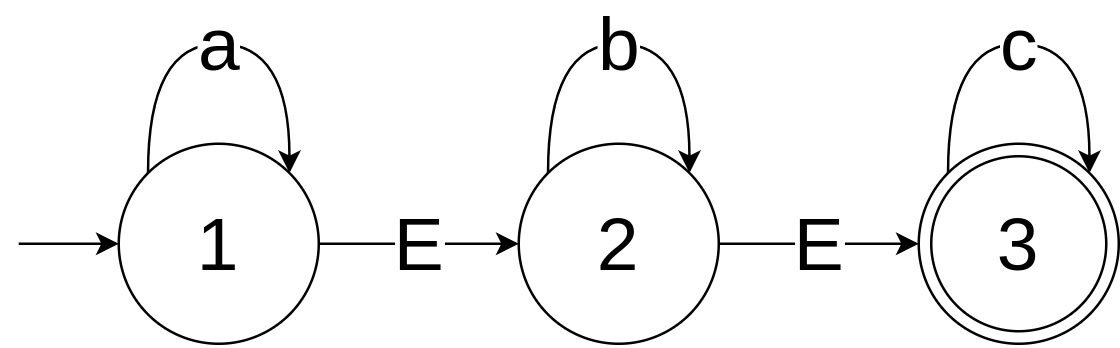
\includegraphics[width=2in]{../EXP5/diagram-ques.png}
	\caption{$\epsilon$-NFA}
\end{figure}

\begin{figure}[H]
	\centering
	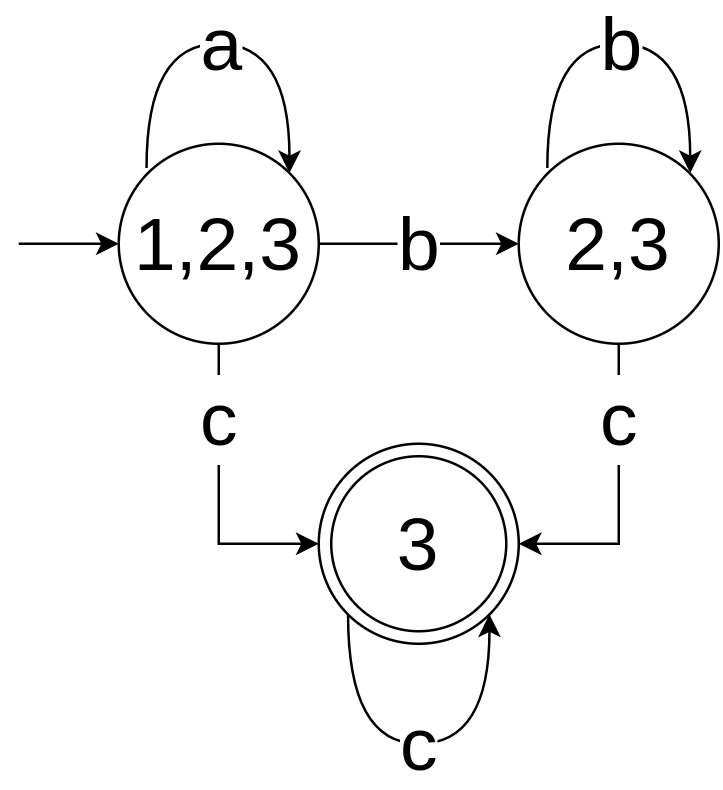
\includegraphics[height=2in]{../EXP5/diagram-ans.png}
	\caption{New NFA}
\end{figure}

\section{Python-Program}
\lstinputlisting[style=CStyle,language=python]{../EXP5/E-NFA_to_NFA.py}

\section{Output}
\lstinputlisting[style=plain]{../EXP5/output.txt}

\section{Result}
The program compiled successfully and converted $\epsilon$-NFA to NFA.


\clearpage
\chapter{Recursive descent parser}

\section{Aim}
To design and construct a recursive descent parser for the given expression.
\begin{algorithmic}[1]
	\State $E\: \quad \rightarrow$ $T \; E’$
	\State $E’  \quad \rightarrow$ $+ \; T \; E’ \; | \; e$
	\State $T\: \quad \rightarrow$ $F \; T’$
	\State $T’  \quad \rightarrow$ $* \; F \; T’ \; | \; e$
	\State $F\: \quad \rightarrow$ $( \; E \; ) \; | \; id$
\end{algorithmic}




\section{Theory}
Top-down parsing can be viewed as the problem of constructing a parse tree for the input string, starting from the root and creating the nodes of the parse tree in pre-order. Equivalently, top-down parsing can be viewed as finding a leftmost derivation for an input string. At each step of a top-down parse, the key problem is that of determining
the production to be applied for a non-terminal. Once an production is chosen, the rest of the parsing process consists of "\textit{matching}" the terminal symbols in the production body with the input string.


Recursive descent parser is a general form of top-down parsing, which may require backtracking to find the correct production to be applied. On the other hand, a special case of recursive-descent parsing where no backtracking is required is call predictive parsing. Predictive parsing chooses the correct production by looking ahead at the input a fixed number
of symbols.

A recursive-descent parsing program consists of a set of procedures, one for each
non-terminal. Execution begins with the procedure for the start symbol, which halts and announces success if its procedure body scans the entire input string.
General recursive-descent may require backtracking; that is, it may require
repeated scans over the input.

\section{Algorithm}

\begin{algorithm}[H]
	\caption{Non-predictive recursive descent parser without backtracking}
	\begin{algorithmic}[1]
		\Procedure{A}{ }\Comment{A : Non-terminal of grammar}
			
			\State Choose an A-production, $A \gets X X . . . X_k$
					
			\For{$ i = 1$ to $k$}
				\If{$X_i$ is a nonterminal}
					\State Call procedure \Call{$X_i$}{ }
				\ElsIf{$X_i$ equals to the current input symbol $a$}
					\State Advance the input to the next symbol
				\Else
					\State Error Occurred
				\EndIf
			\EndFor
		\EndProcedure
		\State \Call{StartSymbol}{ } \Comment{Call start symbol to
		 start parsing}		
	\end{algorithmic}
\end{algorithm}

\begin{algorithm}[H]
	\caption{Non-predictive recursive descent parser with backtracking}
	\begin{algorithmic}[1]
		\Procedure{A}{ }\Comment{A : Non-terminal of grammar}
		
			\State $inputState \gets CurrentInputState$ 
			\ForAll{production $P=X X . . . X_k \in A-productions$}
				\State $backtrack =$ FALSE
				\For{$ i = 1$ to $k$}
					\If{$X_i$ is a nonterminal}
						\State Call procedure \Call{$X_i$}{ }
					\ElsIf{$X_i$ equals to the current input symbol $a$}
						\State Advance the input to the next symbol
					\Else \Comment{Error occurred, iterate to next production}
						\State $backtrack = TRUE$ 
						\State $break$
					\EndIf
				\EndFor
				\If{$bracktrack = TRUE$}
					\State $input \gets inputState$ \Comment{Restore input status}
				\Else \Comment{Completely parsed a production}
					\State $break$
				\EndIf
			\EndFor
		\EndProcedure
		\State \Call{StartSymbol}{ } \Comment{Call start symbol to start parsing}		
	\end{algorithmic}
\end{algorithm}

\begin{figure}[!h]
	\centering
	
\includegraphics[height=3in]{../EXP6/diagram.png}
	\caption{Top down parser for id+id*id}
\end{figure}

\break
\section{C-Program}
\lstinputlisting[style=CStyle,language=C]{../EXP6/recursive_descent.c}

\section{Output}
\textbf{Output1}
\lstinputlisting[style=plain]{../EXP6/output1.txt}
\textbf{Output2}
\lstinputlisting[style=plain]{../EXP6/output2.txt}

\section{Result}
The program compiled and successfully parsed an given expression via non predictive recursive descent with backtracking.
\clearpage
\chapter{Shift Reduce Parser}

\section{Aim}
To design and construct a Shift Reduce Parser for a given language
\begin{algorithmic}[1]
	\State $E \quad \rightarrow \quad E \; + \; E$
	\State $E \quad \rightarrow \quad E \; - \; E$
	\State $E \quad \rightarrow \quad E \; * \; E$
	\State $E \quad \rightarrow \quad ( \; E \; )$
	\State $E \quad \rightarrow \quad i$
\end{algorithmic}




\section{Theory}
Shift-reduce parsing is a form of bottom-up parsing in which a stack holds
grammar symbols and an input buffer holds the rest of the string to be parsed.
The handle always appears at the top of the stack just before
it is identified as the handle.
A special symbol \$ to mark the bottom of the stack and also the right end of the
input. 

Initially, the stack is empty, and the string $w$ is on the input. During a left-to-right scan of the input string, the parser shifts zero or more
input symbols onto the stack, until it is ready to reduce a string of grammar
symbols on top of the stack. It then reduces to the head of the appropriate production. The parser repeats this cycle until it has detected an error or until
the stack contains the start symbol and the input is empty. Upon entering this configuration, the parser halts and announces successful
completion of parsing.

There are four possible actions a shift-reduce parser can make
\begin{enumerate}
	\item \textbf{Shift}.  Shift the next input symbol onto the top of the stack.
	\item \textbf{Reduce}. The right end of the string to be reduced must be at the top of
the stack. Locate the left end of the string within the stack and decide
with what nonterminal to replace the string.
	\item \textbf{Accept}. Announce successful completion of parsing.
	\item \textbf{Error}. Discover a syntax error and call an error recovery routine.
\end{enumerate}


\section{Algorithm}

\begin{algorithm}[!h]
	\caption{Computation of CLOSURE}
	\label{alg:closure}
	\begin{algorithmic}[1]
		\Procedure{CLOSURE}{I} \Comment{Returns set of Items}
			\State $J \gets I$
			\Repeat 
				\ForAll{item $A \rightarrow \alpha.B\beta$}
					\ForAll{production $B \rightarrow \gamma$ of $G$}
						\If{$B \rightarrow .\gamma$ is not in J}
							\State Add $B \rightarrow .\gamma$ to $J$
						\EndIf
					\EndFor
				\EndFor
			\Until{no more items are added to $J$ on one round}
			\State \Return $J$
		\EndProcedure
	\end{algorithmic}
\end{algorithm}

\begin{algorithm}[!h]
	\caption{Computation of the canonical collection of set of LR(0) items}
	\label{alg:LR0Items}
	\begin{algorithmic}[1]
		\Procedure{items}{G'}
			\State $C \gets \{ \Call{CLOSURE}{\{[S\ \rightarrow .S]\}}\}$ 
			\Repeat
			\ForAll{set of items $I \in C$}
				\ForAll{grammar symbol $X$}
					\If{$\Call{GOTO}{I,X}$ is not empty and not in $C$}
						\State Add \Call{GOTO}{I,X} to C
					\EndIf
				\EndFor
			\EndFor
			\Until{no new set of imtes are added to $C$ on a round}
		\EndProcedure
	\end{algorithmic}
\end{algorithm}

\begin{algorithm}[!h]
	\caption{LR-parsing}
	\label{alg:LRparser}
	\begin{algorithmic}[1]
		\State Let $a$ be the first symbol of $W\$$
		\While{1}
			\State Let $s$ be the state on top of the stack
			\If{$\Call{ACTION}{s,a} = shift \quad t$}
				\State push $t$ onto the stack
				\State let $a$ be the next input symbol
			\ElsIf{$\Call{ACTION}{s,a} = reduce \quad A \rightarrow \beta$}
				\State pop $|\beta|$ symbols off the stack
				\State let state $t$ now be on top of the stack
				\State push $\Call{GOTO}{t,A}$ onto the stack
				\State output the production $A \rightarrow \beta$
			\ElsIf{$\Call{ACTION}{s,a} = accept$}
				\State break \Comment{Parsing is done}
			\Else
				\State call error-recovery routine
			\EndIf
		\EndWhile
	\end{algorithmic}
\end{algorithm}

\break

\section{Grammar}
\subsection{Augmented Grammar}
\begin{algorithmic}[1]
	\setcounter{ALG@line}{-1}	
	\State $E' \quad \rightarrow \quad E$
	\State $E \quad \rightarrow \quad E \; + \; E$
	\State $E \quad \rightarrow \quad E \; - \; E$
	\State $E \quad \rightarrow \quad E \; * \; E$
	\State $E \quad \rightarrow \quad ( \; E \; )$
	\State $E \quad \rightarrow \quad i$
\end{algorithmic}

\break
\subsection{LR(0) Automaton}
\begin{figure}[!h]
	\centering
	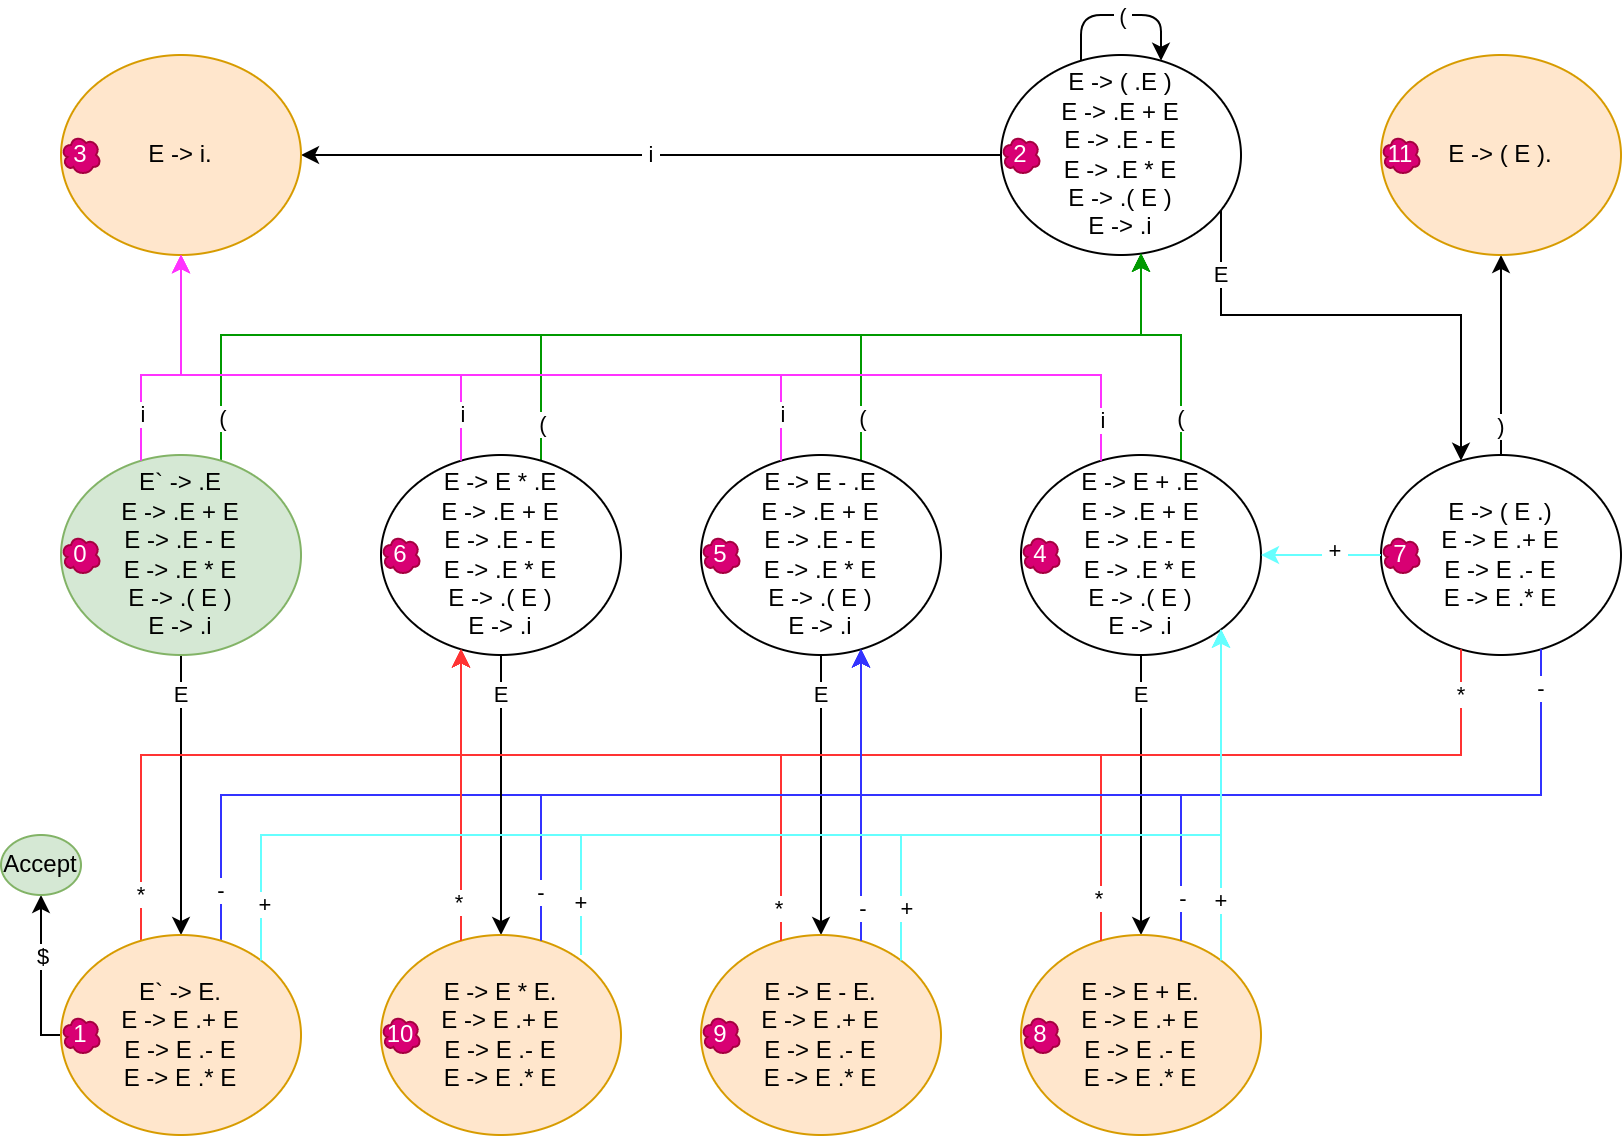
\includegraphics[width=\textwidth]{../EXP7/automaton.png}
	\caption{LR(0) Automaton}
\end{figure}

\subsection{First \& Follow}
\begin{table}[!h]
	\centering
	\begin{tabular}{|lll|}
		\hline
		\multicolumn{3}{|c|}{\textbf{FIRST / FOLLOW table}}                      \\ \hline
		\multicolumn{1}{|c|}{\textbf{Nonterminal}} & \multicolumn{1}{c|}{\textbf{FIRST}} & \multicolumn{1}{c|}{\textbf{FOLLOW}} \\ \hline
		\multicolumn{1}{|l|}{E'} & \multicolumn{1}{l|}{\{(,i\}} & \{\$\}         \\ \hline
		\multicolumn{1}{|l|}{E}  & \multicolumn{1}{l|}{\{(,i\}} & \{\$,+,-,*,)\} \\ \hline
	\end{tabular}
\end{table}

\break
\subsection{Parse-Table}
\begin{table}[!h]
	\centering
	\resizebox{\textwidth}{!}{%
		\begin{tabular}{|cccccccccc|}
			\hline
			\multicolumn{10}{|c|}{\textbf{LR table}} \\ \hline
			\multicolumn{1}{|c|}{} &
			\multicolumn{7}{c|}{\textbf{ACTION}} &
			\multicolumn{2}{c|}{\textbf{GOTO}} \\ \cline{2-10} 
			\multicolumn{1}{|c|}{\multirow{-2}{*}{\textbf{State}}} &
			\multicolumn{1}{c|}{\textbf{+}} &
			\multicolumn{1}{c|}{\textbf{-}} &
			\multicolumn{1}{c|}{\textbf{*}} &
			\multicolumn{1}{c|}{\textbf{(}} &
			\multicolumn{1}{c|}{\textbf{)}} &
			\multicolumn{1}{c|}{\textbf{i}} &
			\multicolumn{1}{c|}{\textbf{\$}} &
			\multicolumn{1}{c|}{\textbf{E1}} &
			\multicolumn{1}{c|}{\textbf{E}} \\ \hline
			\multicolumn{1}{|c|}{0} &
			\multicolumn{1}{c|}{} &
			\multicolumn{1}{c|}{} &
			\multicolumn{1}{c|}{} &
			\multicolumn{1}{c|}{s2} &
			\multicolumn{1}{c|}{} &
			\multicolumn{1}{c|}{s3} &
			\multicolumn{1}{c|}{} &
			\multicolumn{1}{c|}{} &
			1 \\ \hline
			\multicolumn{1}{|c|}{1} &
			\multicolumn{1}{c|}{s4} &
			\multicolumn{1}{c|}{s5} &
			\multicolumn{1}{c|}{s6} &
			\multicolumn{1}{c|}{} &
			\multicolumn{1}{c|}{} &
			\multicolumn{1}{c|}{} &
			\multicolumn{1}{c|}{acc} &
			\multicolumn{1}{c|}{} &
			\\ \hline
			\multicolumn{1}{|c|}{2} &
			\multicolumn{1}{c|}{} &
			\multicolumn{1}{c|}{} &
			\multicolumn{1}{c|}{} &
			\multicolumn{1}{c|}{s2} &
			\multicolumn{1}{c|}{} &
			\multicolumn{1}{c|}{s3} &
			\multicolumn{1}{c|}{} &
			\multicolumn{1}{c|}{} &
			7 \\ \hline
			\multicolumn{1}{|c|}{3} &
			\multicolumn{1}{c|}{r5} &
			\multicolumn{1}{c|}{r5} &
			\multicolumn{1}{c|}{r5} &
			\multicolumn{1}{c|}{} &
			\multicolumn{1}{c|}{r5} &
			\multicolumn{1}{c|}{} &
			\multicolumn{1}{c|}{r5} &
			\multicolumn{1}{c|}{} &
			\\ \hline
			\multicolumn{1}{|c|}{4} &
			\multicolumn{1}{c|}{} &
			\multicolumn{1}{c|}{} &
			\multicolumn{1}{c|}{} &
			\multicolumn{1}{c|}{s2} &
			\multicolumn{1}{c|}{} &
			\multicolumn{1}{c|}{s3} &
			\multicolumn{1}{c|}{} &
			\multicolumn{1}{c|}{} &
			8 \\ \hline
			\multicolumn{1}{|c|}{5} &
			\multicolumn{1}{c|}{} &
			\multicolumn{1}{c|}{} &
			\multicolumn{1}{c|}{} &
			\multicolumn{1}{c|}{s2} &
			\multicolumn{1}{c|}{} &
			\multicolumn{1}{c|}{s3} &
			\multicolumn{1}{c|}{} &
			\multicolumn{1}{c|}{} &
			9 \\ \hline
			\multicolumn{1}{|c|}{6} &
			\multicolumn{1}{c|}{} &
			\multicolumn{1}{c|}{} &
			\multicolumn{1}{c|}{} &
			\multicolumn{1}{c|}{s2} &
			\multicolumn{1}{c|}{} &
			\multicolumn{1}{c|}{s3} &
			\multicolumn{1}{c|}{} &
			\multicolumn{1}{c|}{} &
			10 \\ \hline
			\multicolumn{1}{|c|}{7} &
			\multicolumn{1}{c|}{s4} &
			\multicolumn{1}{c|}{s5} &
			\multicolumn{1}{c|}{s6} &
			\multicolumn{1}{c|}{} &
			\multicolumn{1}{c|}{s11} &
			\multicolumn{1}{c|}{} &
			\multicolumn{1}{c|}{} &
			\multicolumn{1}{c|}{} &
			\\ \hline
			\multicolumn{1}{|c|}{8} &
			\multicolumn{1}{c|}{\cellcolor[HTML]{FFC0CB}s4 / \sout{r1}} &
			\multicolumn{1}{c|}{\cellcolor[HTML]{FFC0CB}s5 / \sout{r1}} &
			\multicolumn{1}{c|}{\cellcolor[HTML]{FFC0CB}s6 / \sout{r1}} &
			\multicolumn{1}{c|}{} &
			\multicolumn{1}{c|}{r1} &
			\multicolumn{1}{c|}{} &
			\multicolumn{1}{c|}{r1} &
			\multicolumn{1}{c|}{} &
			\\ \hline
			\multicolumn{1}{|c|}{9} &
			\multicolumn{1}{c|}{\cellcolor[HTML]{FFC0CB}s4 / \sout{r2}} &
			\multicolumn{1}{c|}{\cellcolor[HTML]{FFC0CB}s5 / \sout{r2}} &
			\multicolumn{1}{c|}{\cellcolor[HTML]{FFC0CB}s6 / \sout{r2}} &
			\multicolumn{1}{c|}{} &
			\multicolumn{1}{c|}{r2} &
			\multicolumn{1}{c|}{} &
			\multicolumn{1}{c|}{r2} &
			\multicolumn{1}{c|}{} &
			\\ \hline
			\multicolumn{1}{|c|}{10} &
			\multicolumn{1}{c|}{\cellcolor[HTML]{FFC0CB}s4 / \sout{r3}} &
			\multicolumn{1}{c|}{\cellcolor[HTML]{FFC0CB}s5 / \sout{r3}} &
			\multicolumn{1}{c|}{\cellcolor[HTML]{FFC0CB}s6 / \sout{r3}} &
			\multicolumn{1}{c|}{} &
			\multicolumn{1}{c|}{r3} &
			\multicolumn{1}{c|}{} &
			\multicolumn{1}{c|}{r3} &
			\multicolumn{1}{c|}{} &
			\\ \hline
			\multicolumn{1}{|c|}{11} &
			\multicolumn{1}{c|}{r4} &
			\multicolumn{1}{c|}{r4} &
			\multicolumn{1}{c|}{r4} &
			\multicolumn{1}{c|}{} &
			\multicolumn{1}{c|}{r4} &
			\multicolumn{1}{c|}{} &
			\multicolumn{1}{c|}{r4} &
			\multicolumn{1}{c|}{} &
			\\ \hline
		\end{tabular}%
	}
\end{table}


\subsection{Parse-Tree}
\begin{figure}[!h]
	\centering
	
\includegraphics[height=2in]{../EXP7/parse_tree.png}
	\caption{Bottom up parser for i+i*i}
\end{figure}

\break
\section{C-Program}
\lstinputlisting[style=CStyle,language=C]{../EXP7/shiftreducer.c}

\section{Output}
Output1
\lstinputlisting[style=plain]{../EXP7/output1.txt}
Output2
\lstinputlisting[style=plain]{../EXP7/output2.txt}

\section{Result}
The program compiled and successfully parsed a string via Simple LR parser for the given grammar.

%\printbibliography
\end{document}
